
\documentclass[fleqn]{hw}

\usepackage{notes}
\usepackage{url}
\usepackage{graphicx}
\usepackage{amsmath}
\usepackage{float}
\topmargin -1.5cm        % read Lamport p.163
\oddsidemargin -0.04cm   % read Lamport p.163
\evensidemargin -0.04cm  % same as oddsidemargin but for left-hand pages
\textwidth 16.59cm
\textheight 21.94cm
\parskip 7.2pt           % sets spacing between paragraphs

\newcommand{\indep}{\perp}

\title{HW5: Bayesian Networks \& Independence}
\class{CS6300: Artificial Intelligence, Spring 2018}
\institute{University of Utah}
\author{Jake Pitkin}
% IF YOU'RE USING THIS .TEX FILE AS A TEMPLATE, PLEASE REPLACE
% The author WITH YOUR NAME AND UID.
% Replace the due date with anyone you worked with i.e. "Worked with: John McCarthy, Watson, & Hal-9000"
\begin{document}
\maketitle

\section{Independences from Probability Tables}

\begin{table}[H]
\centering	
\begin{tabular}{|ccc|c|}
\hline
{\bf A} & {\bf B} & {\bf C} & $p$ \\
\hline
T & T & T & $1/16$ \\
T & T & F & $1/3$ \\
T & F & T & $1/32$ \\
T & F & F & $1/12$ \\
F & T & T & $3/16$ \\
F & T & F & $1/6$ \\
F & F & T & $3/32$ \\
F & F & F & $1/24$ \\
\hline
\end{tabular}
\caption{$P(A, B, C)$}
\end{table}

I considered a few factorizations and found one that satisfied the above table.

\begin{center}
	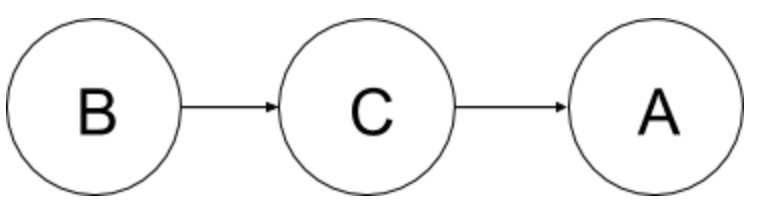
\includegraphics[width=0.25\textwidth]{p1}
\end{center}

This factorizes the joint probability $P(A, B, C)$ as a product of the conditional probabilities $P(B)$, $P(C | B)$, and $P(A | C)$. 

\begin{table}[H]
        \begin{minipage}{0.333\textwidth}
            \centering
            \begin{tabular}{|c|c|}
\hline
{\bf B} & $p$ \\
\hline
T & $3/4$ \\
F & $1/4$ \\
\hline
\end{tabular}
\caption{$P(B)$}
        \end{minipage}
        \begin{minipage}{0.3333\textwidth}
            \centering
      \begin{tabular}{|cc|c|}
\hline
{\bf C} & {\bf B} & $p$ \\
\hline
T & T & $1/3$ \\
T & F & $1/2$ \\
F & T & $2/3$ \\
F & F & $1/2$ \\
\hline
\end{tabular}
\caption{$P(C | B)$}
        \end{minipage}
        \begin{minipage}{0.333\textwidth}
            \centering
\begin{tabular}{|cc|c|}
\hline
{\bf A} & {\bf C} & $p$ \\
\hline
T & T & $1/4$ \\
T & F & $2/3$ \\
F & T & $3/4$ \\
F & F & $1/3$ \\
\hline
\end{tabular}
\caption{$P(A | C)$}
        \end{minipage}
    \end{table}
    
With 10 total entries, this is the smallest you can get the conditional probability tables (keeping the graph connected). These were derived by marginalizing out variables from $P(A, B, C)$ and using the product rule for dependent variables.

\newpage
\section{Independence in Graphical Models}

Consider the graphical model shown below:

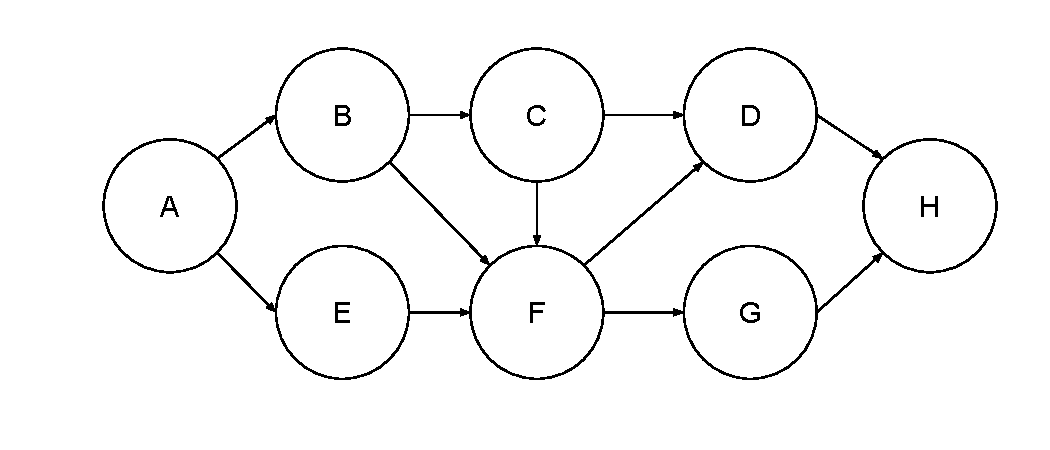
\includegraphics[width=0.5\textwidth]{example-network}

Please answer the following conditional independence questions from
this model:

\begin{enumerate}
\item $A \indep H$ - {\bf No}: There is an active path between $A$ and $H$ by causal chain.
\item $A \indep H | C$ - {\bf No}: There is an active path between $A$ and $H$ by causal chain.
\item $A \indep H | C,F$ - {\bf Yes}: There is no active path between $A$ and $H$.
\item $E \indep B | A$ - {\bf Yes}: There is no active path between $E$ and $B$.
\item $E \indep B | C,F$ - {\bf No}: There is an active path between $E$ and $B$ by common cause. 
\item $E \indep B | A,C,F$ - {\bf No}: There is an active path between $E$ and $B$ by common cause.
\end{enumerate}

\newpage
\section{Inference by Enumeration and Variable Elimination}

The following queries are answered using the probability tables found in the lecture slides.

\begin{enumerate}
\item $p(b, \lnot e | a, j, m)$

\begin{align*}
p(b, \lnot e | a, j, m) &= \frac{p(b, \lnot e, a, j, m)}{p(a, j, m)} \\ \\
&= \frac{p(b) \ p(\lnot e) \ p(j | a) \ p(m | a) \ p(a | b, \lnot e)}{p(j | a) \ p(m | a) \ \sum_{b} \sum_{e} p(B) \ p(E) \ p(a | B, E)} \\ \\
&= \frac{0.001 * 0.998 * 0.9 * 0.7 * 0.94}{0.9 * 0.7 * (0.001 * 0.002 * 0.95 + 0.999 * 0.002 * 0.29 \ + } \\
&\qquad\qquad\qquad \ 0.001 * 0.998 * 0.94 + 0.999 * 0.998 * 0.001) \\ \\
&= \frac{0.0005910156}{0.00158535846} \\ \\
&= {\bf 0.372796}
\end{align*}

\item $p(b | a)$

\begin{align*}
p(b|a) &= \frac{\sum_{e} \sum_{j} \sum_{m} p(b) \ p(E) \ p(a | b, E) \ p(J | a) \ p(M | a)}{\sum_{b} \sum_{e} \sum_{j} \sum_{m} p(E) \ p(E) \ p(a | B, E) p(J | a) \ p(J | a)} \\ \\
&= \frac{p(b) \sum_{e} p(E) \ p(a | b, E)}{\sum_{b} \sum_{e} p(B) \ p(E) \ p(a|B, E)} \\ \\
&= \frac{0.001 * (0.002 * 0.95 + 0.998 * 0.94)}{0.001 * 0.002 * 0.95 + 0.999 * 0.002 * 0.29 + 0.001 * 0.998 * 0.94 + 0.999 * 0.998 * 0.001} \\ \\
&= \frac{0.00094002}{0.002516442} \\ \\
&= {\bf 0.3735512}
\end{align*}

\newpage
\item $p(b | e,a)$  (how does this compare to the previous one?)

\begin{align*}
p(b | e, a) & = \frac{\sum_{j} \sum_{m} p(b) \ p(e) \ p(a | b, e) \ p(J | a) \ p(M | a)}{\sum_{b} \sum_{j} \sum_{m} p(B) \ p(e) \ p(a | B, e) p(J | a) \ p(M | a)} \\ \\ 
&= 	\frac{p(b) \ p(e) \ p(a | b, e)}{p(e) \sum_{b} p(B) \ p(a|B, e)} \\ \\
&= \frac{0.001 * 0.002 * 0.95}{0.002 * (0.001 * 0.95 + 0.999 * 0.29)} \\ \\
&= \frac{0.0000019}{0.00058132} \\ \\ 
&= {\bf 0.0032684}
\end{align*}

This makes sense. If there is an earthquake and the alarm is going off, it's unlikely that there is a burglary occurring at the same moment. But in question 2, we know only the alarm is going off and there is a much larger chance there is a burglary occurring (causing the alarm to go off).

\item $p(a | j,\lnot m)$

Note: in the numerator I take the result of marginalizing {\it b} and {\it e} when {\it a} is true from question 1 rather than showing the work again. For denominator I solved it using Excel.

\begin{align*}
p(a | j, \lnot m) & = \frac{p(j | a) \ p(\lnot m | a) \ \sum_{b} \sum_{e} p(B) \ p(E) \ p(a | B, E)}{\sum_{b} \sum_{e} \sum_{a} p(B) \ p(E) \ p(A | B, E) p(j | A) \ p(\lnot m | A)} \\ \\ 
&= \frac{0.9 * 0.01 * 0.002516442}{\sum_{b} \sum_{e} p(B) \ p(E) \ f(B, E, j, \lnot m)}
\end{align*}

\begin{align*}
\qquad \qquad \quad &= \frac{0.000226479}{0.0500548} \\ \\
&= {\bf 0.0045246}
\end{align*}


\end{enumerate}

Now, repeat items (2) and (4) using variable elimination.  When you
have to choose a variable to eliminate, choose alphabetically.

\begin{enumerate}
\item[2.] $p(b | a)$
\item[4.] $p(a|j, \lnot m)$	
\end{enumerate}


\end{document}
